 \documentclass[reprint,
superscriptaddress,
amsmath,amssymb,aps,showkeys,showpacs,
twoside,final,secnumarabic,%raggedbottom,
nofootinbib]{revtex4-2}

%======Размеры бумаги и~текста=======
\usepackage[paperwidth=205mm,paperheight=290mm,top=17mm,bottom=25mm,
%,16mm,% inner=18mm,% outer=15mm,
inner=17mm,outer=17mm,
twoside]{geometry}

%================Пакеты=====================
\usepackage{cmap} % Улучшенный поиск %русских слов в~полученном pdf-файле
\defaulthyphenchar=127 % Если стоит до fontenc, то переносы не впишутся в~выделяемый текст при копировании его в~буфер обмена
\usepackage[T1,T2A]{fontenc}
\usepackage[utf8]{inputenc}
%\usepackage[cp1251]{inputenc}
\usepackage[russian,english]{babel}
\usepackage{color}
%\usepackage{physics}
\usepackage{graphicx}% Include figure files
\usepackage{dcolumn}% Align table columns on decimal point
\usepackage{bm} % bold math
\usepackage[unicode=true,colorlinks=true,linkcolor=magenta, urlcolor=blue, citecolor = blue,breaklinks]{hyperref}
% add hypertext capabilities
\usepackage{multirow}
\usepackage{url}
\def\UrlBreaks{\do\/\do-}
\usepackage{breakurl}
%\usepackage{float}
\newcommand\sbullet[1][.5]{\mathbin{\vcenter{\hbox{\scalebox{#1}{$\bullet$}}}}}
%========Для работы на компе==================
%\usepackage{../latex/breakurl}
%\graphicspath{{../figures/}}
\DeclareGraphicsExtensions{.eps}

%===========Счетчики================
\newcount\issue
\newcount\Vol
\newcount\numb
% ======Колонтитулы==============
\headheight=1.5cm
\usepackage{fancyhdr} %this packages %provides fancy up and bottom of page
\pagestyle{fancy}
\fancyhead{}\fancyfoot{}
%\footheight=0.5cm
\fancyfoot[LO]{}
\fancyfoot[CO]{\small{\numb--\thepage}}
\fancyfoot[RO]{}
\fancyfoot[LE]{}
\fancyfoot[CE]{\small{\numb--\thepage}}
\fancyfoot[RE]{}
\fancyhead[CO]{\normalsize\textrm{Moscow University Physics Bulletin \Vol(\the\issue)},~\numb~(\the\year)}
% {текст-центр-нечетные}

\fancyhead[CE]{\normalsize\selectlanguage{english}{Modern Machine Learning Methods}}
% {текст-центр-четные}

%=======Ссылка на почту=======
\newcommand\mailto[1]{\href{mailto:#1}{#1}}
%============================
\renewcommand\thesection{\arabic{section}}
\renewcommand\thetable{\arabic{table}}

%============================
\year2023 \issue7
%\sheets999
\def\Vol{\textbf{78}}
\def\numb{x}
\setcounter{page}{1}
%============================

\begin{document}

%====== Начало шапки статьи  ============
\title{MODERN MACHINE LEARNING METHODS\\[20pt]
Hyper-parameter tuning of neural network for\\
high-dimensional problems in the case of Helmholtz equation}

\def\address{Department of Computational Physics, St. Petersburg State University,\\
1 Ulyanovskaya Street, St-Petersburg, Russia}

\author{\firstname{D.N.}~\surname{Polyakov}}
\email[E-mail: ]{daniil.polyakov.2001@gmail.com}
\affiliation{\address}
\author{\firstname{M.M.}~\surname{Stepanova}}
\email[E-mail: ]{m.stepanova@spbu.ru}
\affiliation{\address}

\received{xx.xx.2023}
\revised{xx.xx.2023}
\accepted{xx.xx.2023}

\begin{abstract}
In this work we study the effectiveness of common hyper-parameter optimization (HPO) methods for physics-informed neural network (PINN) with application to multidimensional Helmholtz problem. The network was built upon PyTorch framework without the use of special PINN-oriented libraries. We investigate the effect of hyper-parameters on NN model performance and conduct automatic hyper-parameter optimization using different combinations of search algorithms and trial schedulers.
We chose an open-source HPO framework Ray Tune that provides unified interface for many HPO packages as the HPO tool in our work. We consider two search algorithms: random search and Bayesian method based on tree-structured Parzen estimator (TPE), in implementations hyperopt and hpbandster, and the Asynchronous Successive Halving (ASHA) early-stopping algorithm. For our problem, enabling early-stopping algorithm is shown to achieve faster HPO convergence speed than switching from random search to Bayesian method.
\end{abstract}

\pacs{02.60.Cb, 02.60.Pn, 02.70.$-$c, 02.90.+p}\par
\keywords{HPO, PINN, Helmholtz equation, PyTorch, Ray Tune\\[5pt]}
%DOI:  

\maketitle
\thispagestyle{fancy}

%====== Начало  статьи  ============

\section{Introduction}
Traditional classes of methods for numerical solving of differential equations are the finite difference methods (FDM) and the finite element methods (FEM) \cite{bib01}. These techniques have been evolving over the decades, and as a result, powerful algorithms for modeling various physical processes have been developed. However, these methods have disadvantages, such as discretization errors and exponential growth of computing resources requirements with an increase of the dimensionality of the problem.

In recent years, more and more theoretical and applied problems are being solved using deep learning methods \cite{bib02,bib03,bib04,bib05}.

In particular, since the neural network is a universal approximator \cite{bib06}, it can be used to approximate functions and solve differential equations. In \cite{bib07}, a class of physics-informed neural networks (PINNs) oriented towards solving partial differential equations (PDEs) is introduced. The idea is to incorporate the equation being solved into the objective function of the neural network. In this case, the derivative of the objective function with respect to the network parameters can be calculated analytically, relying on automatic differentiation. Multiple open-source libraries implementing PINNs have already been developed \cite{bib08}.

The advantage of neural networks over FDM and FEM is their ability to generalize, i.e., to predict a solution in a domain outside the training sample. In \cite{bib09} authors present the solution of a two-dimensional wave equation using a neural network trained on a sample taken at the initial time. The resulting network gives a good approximation of the solution at subsequent time steps.

To obtain the best result, before training the model, it is necessary to correctly configure its hyper-parameters. Hyper-parameters of a neural network refer to parameters that do not get updated during model training. These can be parameters related to the model architecture, such as the number of hidden layers, layer width, and activation function, or parameters related to the learning process of the model, such as learning rate, batch size, optimizer and its possible parameters. Hyper-parameters determine the rate of convergence of the model and its maximum possible accuracy.

The process of selecting the model configuration is often very time consuming. In this regard, research and development is currently underway in the field of automatic hyper-parameter optimization (HPO) \cite{bib10}. Although reducing human efforts, HPO demands a large amount of computational resources, especially when several hyper-parameters are optimized together. Study \cite{bib11} presents an example of an HPO procedure for solving the two-dimensional Helmholtz equation.

In this study, we explore the procedures of manual and automatic optimization of neural network hyper-parameters for solving the Helmholtz equation in high-dimensional domains (up to 8). We also perform the comparison of the HPO methods. The NN model is built and trained with PyTorch framework without the use of any special libraries for PINN networks, and automatic HPO is carried out using the Ray Tune framework.

\section{Theory}

\subsection{Physics-informed neural networks}

\paragraph{Problem statement.}
Artificial neural networks may be applied to solve PDEs of the form \cite{bib08}:
\begin{gather*}
f \left(\mathbf{x}; u; \frac{\partial u}{\partial x_1}, \cdots, \frac{\partial u}{\partial x_n}; \frac{\partial^2 u}{\partial x_1 \partial x_1}, \cdots, \frac{\partial^2 u}{\partial x_1 \partial x_n}, \cdots \right) = 0\\
\mathbf{x} \in \Omega, \quad \Omega \subset \mathbb{R}^n
\end{gather*}
with suitable boundary conditions
\[\mathcal{B}(\mathbf{x}, u)|_{\partial \Omega} = 0\]
where $\mathcal{B}(\mathbf{x}, u)$ could be Dirichlet, Neumann, Robin, or periodic boundary conditions.

The key feature of using a neural network as an approximating function for $u(\mathbf{x})$ is the ability to analytically calculate derivatives with respect to $\mathbf{x}$.

\paragraph{Objective function.}
As a measure of the error and as the loss function, we can use the weighted sum of $L^2$ norms of deviations (residuals) for the domain and the boundary:
\[\mathrm{loss} = \omega_f \mathrm{loss}_f + \omega_\mathcal{B} \mathrm{loss}_\mathcal{B}\]
\begin{align*}
\mathrm{loss}_f &= \frac{1}{|N_f|} \sum \limits_{x \in N_f} \left\Vert f \left( \mathbf{x}; \hat{u}; \frac{\partial \hat{u}}{\partial x_1}, \cdots, \frac{\partial^2 \hat{u}}{\partial x_n \partial x_n} \right) \right\Vert^2\\
\mathrm{loss}_\mathcal{B} &= \frac{1}{|N_\mathcal{B}|} \sum \limits_{x \in N_\mathcal{B}} \left\Vert \mathcal{B}(\mathbf{x}, \hat{u}) \right\Vert^2
\end{align*}
where $\omega_f$, $\omega_\mathcal{B}$ — weights; $N_f = \lbrace x_1, \ldots, x_{|N_f|} \rbrace$, $N_\mathcal{B} = \lbrace x_1, \ldots, x_{|N_\mathcal{B}|} \rbrace$ — sets of collocation points (training sample) for the domain and the boundary, respectively; $|N_f|$, $|N_\mathcal{B}|$ — number of points; $\hat{u}$ — NN solution.

In the case of the simplest boundary conditions, when $u|_{\partial \Omega} = g(x)$, $\Omega = [a, b]^n$, one can enforce hard constraint by multiplying the output of the neural network by a smooth function that satisfies these conditions:
\[\tilde{u} = g(x) + u \cdot \prod \limits_i^n (x_i - a)(b - x_i)\]

Then the boundary collocation points are no longer needed, and only the term responsible for the discrepancy on the domain remains in the objective function($\mathrm{loss}_f$).

\subsection{Hyper-parameters}
Hyper-parameters can be divided into two groups: those related to model architecture and those related to training. Typical architectural NN parameters are the number of layers, the layer width, and the activation function. These hyper-parameters affect the ability of the model to learn, i.e. its maximum possible accuracy and ability to generalize. The choice of hyper-parameters associated with the training of the model mostly affects the speed of its training. Typical such parameters are learning rate, batch size and the optimizer.

\paragraph*{Learning rate.}
Learning rate (LR) is a positive scalar that specifies the step size during gradient descent. In most cases, this parameter must be adjusted during model training in order to achieve better model accuracy. As a general rule, training should start with high LR value and be reduced over time. This can be done manually, or using a scheduler that automatically adjusts LR during training process. In such a case, LR can be a function of the training epoch, the time, or the value of the loss function.

Possible implementations of the scheduler: linear LR decay; exponential LR decay; step-based LR decay; cyclic schedule; LR reduction on plateau.

The choice of the optimal LR value or the parameters of its scheduler is a complex task. A small LR value leads to slow convergence, while a large LR value prevents convergence. Furthermore, the optimal parameters of the LR scheduler depend on the selected optimizer \cite{bib12}, so they should be adjusted accordingly.

\paragraph*{Batch size.}
The aim of mini-batch gradient descent is to solve the following two problems \cite{bib13}. Compared with standard gradient descent, mini-batch gradient descent accelerates the training process, especially on a large dataset. Compared with SGD with a mini-batch size of 1, mini-batch gradient descent reduces the noise and increases the probability of convergence \cite{bib14}. The maximum batch size is limited by the available memory of the device on which the model is being trained.

There is a correlation between the optimal values of the batch size and the learning rate: the larger the batch size, the greater the corresponding optimal value of the learning rate.

\paragraph*{Optimizer.}
The basic NN optimization method is Stochastic Gradient Descent (SGD). This optimizer tends to oscillate around a local minimum, so its modified version is often used instead: SGD with momentum \cite{bib15}. The momentum value is also a hyper-parameter. Introducing momentum reduces the oscillation by strengthening the update in the same direction and decreasing the change in different directions .

Other common optimizers are Adagrad \cite{bib16}, Root mean square prop (RMSprop) \cite{bib17}, Adaptive momentum estimation (Adam) \cite{bib18}. In applied problems, Adam is recommended to be used by default when training deep neural networks \cite{bib19}. Although this algorithm has more hyper-parameters than other optimizers, it performs well at default values.

\paragraph*{Number of hidden layers.}
Deep neural networks with a great number of hidden layers usually have more potential to learn and achieve better accuracy. Adding layers is a typical method for improving model accuracy \cite{bib20}.

\paragraph*{Layer width.}
On the one hand, a very small number of neurons in the hidden layer leads to a “weak” model, which is unable to approximate the relationship between input and output data. On the other hand, a large number of neurons increases the training time and can lead to overfitting.

\paragraph*{Regularization.}
As the number of layers and neurons increases, the problem of overfitting arises, where the model performance improves on the training dataset, while worsening on the test dataset. To solve this problem, regularization methods are used when, together with minimizing the objective function, they try to minimize the absolute values of the model parameters $\theta$. The regularization term $w^\ast$ is added to the objective function with some coefficient $\lambda$:
\[\mathrm{loss}^\ast = \mathrm{loss} + \lambda w^\ast\]

Typical regularization terms:
\begin{center}
L1: $w^\ast = \sum \limits_i |\theta_i|$ \quad or \quad L2: $w^\ast = \sum \limits_i \theta_i^2$
\end{center}

$\lambda$ values that are too large may lead to oversimplification of the network, and $\lambda$ values that are too small may not solve the overfitting problem. Therefore, this coefficient is another hyper-parameter to be optimized.

\paragraph*{Activation function.}
Activation functions are essential in deep learning because they introduce non-linearity in the output of neurons. Without activation functions, the neural network turns out to be a linear regression model that is unable to represent the complex relationship between the data. Activation functions must be differentiable so that derivatives can be calculated and gradient descent can be performed over all network parameters. Examples of the most common activation functions: sigmoid, hyperbolic tangent, ReLU and its variations. More specific activation functions include sine and arc tangent, which can be useful in solving the problem presented in this study.

\subsection{Hyper-Parameter Optimization}
HPO consists of two main components:
\begin{itemize}
\item \textit{search algorithm} — samples the points from hyper-parameter space for evaluation;
\item \textit{trial scheduler} — stops the model training process in advance in case of poor convergence compared to previous results.
\end{itemize}

Training a neural network is a resource-intensive process. The convergence rate of the model is determined by the choice of its hyper-parameters, and in the case of a non-optimal configuration, it is advisable to interrupt training and move on to another configuration. However, it is important to avoid abandoning a potentially good configuration. To automate this procedure, trial schedulers (early stopping algorithms) are used. These algorithms compare the training dynamics for different configurations with each other and decide whether to temporarily pause or abandon training of particular configuration.
 
\subsubsection{Search algorithms}

\paragraph*{Grid search.}
The most basic search method is grid search. It performs an exhaustive search over a given hyper-parameter set. The user chooses the points to be evaluated, which means he should have some understanding of the influence of hyper-parameters on the result. Such a search is applicable only for a small number of hyper-parameters. As the number of hyper-parameters increases, the number of points grows exponentially (the “curse of dimensionality”).

The grid search can be done in parallel because all points are known in advance.

\paragraph*{Random search.}
An improvement over grid search is random search. In this case, evaluation points are sampled randomly from specified distributions. The search process continues until the required accuracy is obtained, or until the allocated resources expire. This method provides faster convergence compared to grid search, especially for a large number of search space dimensions.

Random search can be done in parallel because the sampling of each subsequent point is performed independently of the previous one.

\paragraph*{Bayesian optimization.}
Bayesian optimization is a sequential iterative algorithm based on two components: \textit{probability surrogate model} and \textit{acquisition function}. At each iteration, the surrogate model is fitted to all accumulated observations of the objective function. The initial set of points is sampled randomly. Based on this model, the acquisition function chooses the next evaluation point, trying to balance exploration and exploitation to avoid trapping into the local optimum.

The surrogate model is used to express the hypothetical form of the objective function. There are many variants of such models \cite{bib21}, but traditionally \textit{Gaussian process} (GP) is used \cite{bib22}. Another popular model is the \textit{Tree Parzen Estimator} (TPE) \cite{bib23}. Unlike GP that works with continuous search spaces, TPE can be used to process categorical and conditional spaces efficiently, and therefore TPE may be more suitable for HPO tasks.

Among acquisition functions, the \textit{expected improvement} algorithm \cite{bib24} is definitely the most common choice:
\[\mathbb{E}[\mathbb{I}(\mathbf{\lambda})] = \mathbb{E}[\max(f_{\min} - y, 0)]\]
where $\mathbb{I}(\mathbf{\lambda})$ — improvement function, $\lambda$ — point in hyper-parameter space, $y$ — surrogate model, $f_{\min}$ — the best value of the objective function at the moment.

The expected improvement can be calculated analytically if the surrogate model is constructed from a normal distribution.

Bayesian optimization is a resource-intensive algorithm, so it is appropriate to use it only for optimizing rather heavy functions. The problem of HPO in deep learning just satisfies this condition. Another disadvantage of the method is it being sequential due to the rebuilding of the surrogate model after each iteration. For this reason, the algorithm is not subject to parallelization, which, nevertheless, can be implemented by resorting to a distortion of the algorithm and a decrease in its efficiency.

\subsubsection{Trial schedulers}

\paragraph*{Median stopping.}
Median stopping is the most straightforward early termination policy. A trial is stopped at step $t$ if the best objective value by this step is worse than the median value of the running average of all completed trials' objective values reported at step $t$.

\paragraph*{Successive Halving.}
The Successive Halving (SHA) algorithm can be described as follows (Figure \ref{SHA}): users need to set an initial finite budget $B$ per trial (time limit, epochs limit, etc.) and the number of trials $n$, uniformly query all hyper-parameter sets for a portion of initial budget, evaluate the performance of all trials, drop the worse performing half, double the budget for the remaining half, and repeat the whole pipeline until only one trial remains.
\\
\\

\begin{figure}[h]
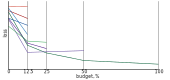
\includegraphics[width=\columnwidth]{img/SHA.pdf}
\caption{Illustration of the successive halving algorithm.}
\label{SHA}
\end{figure}

\paragraph*{HyperBand.}
In SHA, the greater the given number of configurations $n$, the less resources are allocated per configuration at the first stage. Therefore, if the value of $n$ is too large, the training can be aborted too soon, and if the value of $n$ is too small, the number of configurations considered is insufficient. HyperBand (HB) \cite{bib25} is an extension of SHA, mainly designed to solve the “$n$ vs.\ $B/n$” problem. HB puts the SHA inside a loop that varies the values of $B$ and $n$. This measure improves the efficiency of the algorithm.

\paragraph*{Asynchronous Successive Halving.}
Asynchronous Successive Halving (ASHA) \cite{bib26} improves the performance of HB in parallel. In sequential setting, the speed of ASHA is the same as HB.

\paragraph*{BOHB.}
Search algorithms and trial schedulers can work in combination independently of each other. BOHB \cite{bib27} was developed as an attempt to combine Bayesian search and HyperBand into a single efficient algorithm.

\section{Methods}

\subsection{Optimization packages}
We build and train the model using the PyTorch framework. For HPO, we use the Ray Tune framework. Ray Tune provides a unified interface for many popular HPO packages:
\begin{itemize}
\item \textit{search algorithms}: grid search, random search, Ax, BayesOptSearch, BOHB, BlendSearch, CFO, Dragonfly, HEBO, HyperOpt, Optuna, SigOpt, Scikit-Optimize, ZOOpt;
\item \textit{trial schedulers}: ASHA, HyperBand, Median Stopping Rule, Population Based Training (PBT), Population Based Bandits (PB2), BOHB.
\end{itemize}

In this study, search algorithms considered include random search and HyperOpt, which is TPE-based; out of trial schedulers we consider ASHA. We also examine a combined BOHB algorithm.

\subsection{Problem statement}
We employ NN to solve a PDE. The Helmholtz equation was chosen as the equation to be solved:
\begin{gather*}
-\Delta u(\mathbf{x}) - u(\mathbf{x}) = (4 \pi^2 n - 1) \cdot \prod \limits_i^n \sin (2 \pi x_i)\\
u|_{\partial \Omega} = 0
\end{gather*}
where $n$ — domain dimension. The domain is chosen to be a unit hypercube:
\[\Omega = \lbrace \mathbf{x}: \: 0 \leq x_i \leq 1, \: i = 1, \ldots, n \rbrace\]

The right-hand of the equation is chosen so that the solution could be calculated analytically (Figure \ref{analytical_solution}):
\[u(\mathbf{x}) = \prod \limits_i^n \sin (2 \pi x_i)\]
\begin{figure}[h]
\includegraphics{img/analytical solution.png}
\caption{Analytical solution in two-dimensional domain.}
\label{analytical_solution}
\end{figure}

This solution will only be used to verify the correct convergence of the NN, but will not be used during training.

Thus, we need to get a model with $n$ inputs and 1 output that achieves the most accurate solution for the given equation. As a measure of error, we use the root-mean-square error between predicted values of the function and the analytical solution ($\mathrm{RMSE}_u$).

\subsection{NN structure and loss function}
To solve the problem, we build a fully connected feed-forward neural network composed of linear layers of equal width with the same activation functions.

The number of layers $L$, the layer width $N$, and the activation function $\sigma$ are subject to optimization. At the network output, we apply the transformation to enforce the boundary condition:
\[\tilde{u} = u \cdot \prod \limits_i^n (x_i - 0)(1 - x_i)\]

Then the loss function consists only of the discrepancy on the domain:
\begin{flalign*}
&\mathrm{loss} = \mathrm{MSE}_f = & \\
&= \left\langle \left( \Delta u(\mathbf{x}) + u(\mathbf{x}) + (4 \pi^2 n - 1) \cdot \prod \limits_i^n \sin(2 \pi x_i) \right)^2 \right\rangle &
\end{flalign*}

The calculation of the Laplacian of the output value is performed using the \texttt{torch.autograd.grad} method, and vectorized using the \texttt{torch.func.vmap} method. There are several ways to implement the Laplacian, but a combination of these methods was found to be the most efficient.

We do not add the regularization term to the loss function, and we do not consider it as a hyper-parameter in the framework of this study.

\subsection{Collocation points generation}
We generate two sets of collocation points: a training set and a test set. We always sample the equal number of points in both sets. The number of points and the generation method are additional hyper-parameters in our problem. Besides sampling points from a uniform distribution, we also consider the \textit{quasi-random} generation of the training sample. We employ the scrambled Sobol sequence \cite{bib28,bib29} as a quasi-random generator.

PyTorch features the implementation of the Sobol sequence generator that we will be using.

We always sample test points from the classical uniform distribution. All values of equation residual ($\mathrm{MSE}_f$) and solution residual ($\mathrm{RMSE}_u$) displayed in the results below were calculated on the test sample.

\subsection{Hyper-parameter optimization}
The study consists of three parts.

\begin{enumerate}
\item First, we conduct a qualitative study of the influence of hyper-parameters on the convergence of the NN in the cases of 2-dimensional and 5-dimensional problems. We define a configuration grid and conduct a random search over 100 points, allocating equal training time for each point. Then, starting from the obtained optimal configuration, we separate the hyper-parameters into groups and vary them over the grid. After analyzing the results, we choose the optimal values and move on to the next group of hyper-parameters.

\item We compare the automatic HPO algorithms. We examine random search, Bayesian search from the HyperOpt package and the ASHA scheduler in various combinations with each other, as well as the combined BOHB algorithm. For each experiment, we allocate equal time limit per configuration and equal total time limit.

\item Having determined the best combination of HPO algorithms, we run a hyper-parameter search with these algorithms for a 2-, 5-, and 8-dimensional equation. After that, for the best configurations, we train the model until the objective function converges to a plateau.
\end{enumerate}

In the following listed all the hyper-parameters that will be optimized and the corresponding notation used in the tables.

Hyper-parameters, related to training: $|N_f|$ — the number of collocation points in the training set; RNG — training set generation method (random or quasirandom); $|N_\mathrm{batch}|$ — batch size; LR — initial learning rate; LR scheduler — learning rate scheduler.

We consider 4 variants of LR scheduler:\\
$\sbullet[0.5]$ \texttt{None} — no scheduler, i.e. constant LR;\\
$\sbullet[0.5]$ \texttt{ExponentialLR-0.95} (\texttt{ELR-0.95}) — exponential LR scheduler, LR changes by a factor of 0.95 after each iteration;\\
$\sbullet[0.5]$ \texttt{ReduceLROnPlateau-0.1-10} (\texttt{RLRoP-0.1-10}) — LR is multiplied by 0.1, if the objective function does not improve over 11 iterations;\\
$\sbullet[0.5]$ \texttt{ReduceLROnPlateau-0.5-2} (\texttt{RLRoP-0.5-2}) — LR is multiplied by 0.5, if the objective function does not improve over 3 iterations.

Hyper-parameters, related to NN architecture: $N$ — hidden layer width (the number of neurons in the hidden layer); $L$ — the number of hidden layers; $\sigma$ — activation function. We test 5 activation functions: \texttt{ELU} (\textit{exponential linear unit}); \texttt{sigmoid}; \texttt{tanh}; \texttt{sin}; \texttt{atan}.

Other symbols: $i$ — the number of the last training iteration (epoch); $t$ — time limit per configuration; $T$ — total HPO running time; $|N_\mathrm{cfg}|$ — number of evaluated configurations.

The search space in Ray Tune can be specified with different methods. In the present study, four types of distribution are used:\\
$\sbullet[0.5]$ \texttt{choice(a,~b,~c,~\ldots)} — equiprobable choice from the listed values;\\
$\sbullet[0.5]$ \texttt{randint(a,~b)} — sample an integer from a uniform distribution in the interval [a,~b);\\
$\sbullet[0.5]$ \texttt{qlograndint(a,~b,~q)} — sample an integer from the logarithmic distribution in the interval [a,~b] rounded to \texttt{q};\\
$\sbullet[0.5]$ \texttt{qloguniform(a,~b,~q)} — sample a real number from the logarithmic distribution in the interval [a,~b] rounded to \texttt{q}.

Of course, only a random search algorithm samples configurations in exact accordance with the specified distributions. Bayesian methods modify the distributions with surrogate model and sample points using an acquisition function.

\subsection{Computing resources}
NN models were trained on the resources of the Resource 
Center "Computer Center of SPbU". Manual optimization of hyper-parameters (Section \ref{manual_HPO}) was done on an NVIDIA Tesla P100 (16 GB) GPU. Automatic optimization of hyper-parameters and final training of the optimal configuration (Sections \ref{HPO_comparison} and \ref{automatic_HPO}) were done on an NVIDIA RTX A6000 (48 GB) GPU.

\section{Manual HPO on the example of a 5-dimensional problem}\label{manual_HPO}
Search grid is listed in Table \ref{manual_HPO_search_grid}.

\begin{table}[h]
\caption{Search grid and time limit for manual HPO}
\label{manual_HPO_search_grid}
\renewcommand{\arraystretch}{1.25}
\renewcommand{\tabcolsep}{3pt}
\begin{tabular}{|c|p{2in}|}\hline
$N$ & 64, 128, 256, 512, 1024, 2048 \\ \hline
$L$ & 1, 2, 3, 4 \\ \hline
$\sigma$ & \texttt{ELU, sigmoid, tanh, sin, atan} \\ \hline
$|N_f|$ & $10^4, 10^5, 10^6$ \\ \hline
RNG & random (R), quasi-random (QR), \\ \hline
$|N_\mathrm{batch}|$ & 64, 128, 256, 512, 1024, 2048, 4096, 8192, 16384, 32768 \\ \hline
LR & $10^{-4}, 10^{-3}, 10^{-2}, 10^{-1}, 10^0$ \\ \hline
LR scheduler & \texttt{None, ELR-0.95, RLRoP-0.1-10, RLRoP-0.5-2} \\ \hline
$t$ & 300 sec \\ \hline
$|N_\mathrm{cfg}|$ & 100 \\ \hline
\end{tabular}
\end{table}

The best configurations for solving 2- and 5-dimensional problems are presented in Table \ref{manual_HPO_table}.  Dynamics of model training for various hyper-parameters presented in Figure \ref{Dynamics manual}.

Conclusions from manual HPO:
\begin{itemize}
\item Batch size has a relatively low impact on network convergence compared to other parameters. However, very small values slow down training due to parallelization not being utilized and should be avoided.

\item For large LR values, the objective function rapidly declines at the beginning of training, and then acquires an oscillating form. For small LR, convergence is slow, but smoother, and the absolute accuracy of the network is usually higher.

\item Utilizing the LR scheduler is in most cases preferable to a constant LR value, and provides speed and absolute accuracy gains. However, incorrectly selected scheduler parameters can worsen the result.

\item Increasing the number of collocation points does not always improve the speed of convergence, and sometimes even significantly worsens it.

\item The quasi-random sample generation method is superior to the random method, but the gain is small and is usually noticeable when the size of the sample is small.

\item Of the activation functions tested, \texttt{sin} outperforms \texttt{tanh} and greatly outperforms all other functions.

\item For the present problem, the best approximation is achieved by shallow networks with 1–2 hidden layers.
\end{itemize}

The total GPU time spent on manual optimization in the case of a 5-dimensional problem is 24 hours.

\section{Comparison of HPO algorithms on the example of a 5-dimensional problem}\label{HPO_comparison}
In this and the following section we always generate collocation points using a quasi-random method. Search space is listed in Table \ref{HPO_comparison_search_space}.

\begin{table}[h]
\begin{center}\caption{Search grid and time for all HPO alghoritms}
\label{HPO_comparison_search_space}
\renewcommand{\arraystretch}{1.25}
\renewcommand{\tabcolsep}{3pt}
\begin{tabular}{|c|p{2in}|}\hline
$N$ & \texttt{qlograndint(64, 2048, 32)} \\ \hline
$L$ & \texttt{randint(1, 5)} \\ \hline
$\sigma$ & \texttt{choice(ELU, sigmoid, tanh, sin, atan)} \\ \hline
$|N_f|$ & \texttt{choice($10^4, 10^5, 10^6$)} \\ \hline
$|N_\mathrm{batch}|$ & \texttt{qlograndint(64, 32768, 32)} \\ \hline
LR & \texttt{qloguniform(1e-4, 1, 1e-4)} \\ \hline
LR scheduler & \texttt{choice(None, ELR-0.95, RLRoP-0.1-10, RLRoP-0.5-2)} \\ \hline
$t$ & 300 sec \\ \hline
$T$ & 8 hrs \\ \hline
\end{tabular}
\end{center}
\end{table}

Table \ref{HPO_comparison_table} shows the top 3 configurations obtained by each of the HPO algorithms.

\begin{table*}
	\renewcommand{\arraystretch}{1.25}
	\renewcommand{\tabcolsep}{3pt}
	\caption{The best configurations for solving 2- and 5-dimensional problems, obtained manually}
	\label{manual_HPO_table}
	\begin{tabular}{|*{12}{c|}}\hline
		$n$ & $t$, сек & $\mathrm{MSE}_f$ & $\mathrm{RMSE}_u$ & $N$ & $L$ & $\sigma$ & $|N_f|$ & RNG & $|N_\mathrm{batch}|$ & LR & LR scheduler \\ \hline
		2 & 30 & $6.28\mathrm{E}{-4}$ & $7.26\mathrm{E}{-5}$ & 128 & 2 & \texttt{sin} & $10^4$ & QR & 512 & $10^{-2}$ & \texttt{ReduceLROnPlateau-0.1-10} \\ \hline
		5 & 300 & $8.92\mathrm{E}{-2}$ & $1.52\mathrm{E}{-3}$ & 512 & 1 & \texttt{sin} & $10^4$ & QR & 2048 & $10^{-2}$ & \texttt{None} \\ \hline
	\end{tabular}
\end{table*}

\begin{figure*}
	\includegraphics[width=\textwidth]{img/Manual HPO.pdf}
	\caption{Dynamics of model training for various hyper-parameters.}
	\label{Dynamics manual}
\end{figure*}

\begin{table*}
\renewcommand{\arraystretch}{1.25}
\renewcommand{\tabcolsep}{3pt}
\caption{Best configurations obtained by HPO algorithms}
\label{HPO_comparison_table}
\begin{tabular}{|*{13}{c|}}\hline
$|N_\mathrm{cfg}|$ & \verb|#| & $i$ & $t$, sec & $\mathrm{MSE}_f$ & $\mathrm{RMSE}_u$ & $N$ & $L$ & $\sigma$ & $|N_f|$ & $|N_\mathrm{batch}|$ & LR & LR scheduler \\ \hline

\multicolumn{13}{|c|}{Random search} \\ \hline

\multirow{3}{*}{96} & 5 & 107 & 300.1 & $5.0\mathrm{E}{-2}$ & $6.3\mathrm{E}{-4}$ & 1728 & 1 & \texttt{sin} & $10^5$ & 160 & $3.6\mathrm{E}{-1}$ & \texttt{ReduceLROnPlateau-0.5-2} \\ \cline{2-13}

& 10 & 697 & 300.0 & $4.3\mathrm{E}{-1}$ & $1.3\mathrm{E}{-3}$ & 96 & 1 & \texttt{sin} & $10^5$ & 1056 & $2.2\mathrm{E}{-1}$ & \texttt{ReduceLROnPlateau-0.1-10} \\ \cline{2-13}

& 21 & 6 & 304.9 & $3.2\mathrm{E}{-0}$ & $1.3\mathrm{E}{-2}$ & 1088 & 3 & \texttt{sin} & $10^6$ & 128 & $8.0\mathrm{E}{-4}$ & \texttt{None} \\ \hline

\multicolumn{13}{|c|}{Random search + ASHAScheduler} \\ \hline

\multirow{3}{*}{1593} & 364 & 550 & 300.1 & $1.2\mathrm{E}{-2}$ & $2.6\mathrm{E}{-4}$ & 1216 & 1 & \texttt{sin} & $10^5$ & 1760 & $7.9\mathrm{E}{-1}$ & \texttt{ReduceLROnPlateau-0.5-2} \\ \cline{2-13}

& 581 & 1039 & 300.1 & $2.8\mathrm{E}{-2}$ & $2.7\mathrm{E}{-4}$ & 704 & 1 & \texttt{sin} & $10^5$ & 4608 & $9.5\mathrm{E}{-1}$ & \texttt{ReduceLROnPlateau-0.1-10} \\ \cline{2-13}

& 5 & 106 & 300.1 & $4.7\mathrm{E}{-2}$ & $4.4\mathrm{E}{-4}$ & 1728 & 1 & \texttt{sin} & $10^5$ & 160 & $3.6\mathrm{E}{-1}$ & \texttt{ReduceLROnPlateau-0.5-2} \\ \hline

\multicolumn{13}{|c|}{HyperOptSearch} \\ \hline

\multirow{3}{*}{96} & 90 & 277 & 300.2 & $3.3\mathrm{E}{-1}$ & $1.7\mathrm{E}{-3}$ & 768 & 2 & \texttt{sin} & $10^5$ & 928 & $8.1\mathrm{E}{-3}$ & \texttt{ReduceLROnPlateau-0.5-2} \\ \cline{2-13}

& 76 & 1130 & 300.1 & $4.3\mathrm{E}{-1}$ & $1.3\mathrm{E}{-3}$ & 416 & 1 & \texttt{sin} & $10^5$ & 2816 & $2.1\mathrm{E}{-1}$ & \texttt{ReduceLROnPlateau-0.5-2} \\ \cline{2-13}

& 81 & 250 & 300.2 & $5.3\mathrm{E}{-1}$ & $2.1\mathrm{E}{-3}$ & 928 & 2 & \texttt{sin} & $10^5$ & 1408 & $2.0\mathrm{E}{-3}$ & \texttt{ReduceLROnPlateau-0.5-2} \\ \hline

\multicolumn{13}{|c|}{HyperOptSearch + ASHAScheduler} \\ \hline

\multirow{3}{*}{1053} & 817 & 624 & 300.1 & $\mathbf{1.1E{-2}}$ & $\mathbf{1.7E{-4}}$ & 928 & 1 & \texttt{sin} & $10^5$ & 2016 & $1.0\mathrm{E}{-0}$ & \texttt{ReduceLROnPlateau-0.5-2} \\ \cline{2-13}

& 548 & 696 & 300.1 & $1.1\mathrm{E}{-2}$ & $2.3\mathrm{E}{-4}$ & 736 & 1 & \texttt{sin} & $10^5$ & 1824 & $8.6\mathrm{E}{-1}$ & \texttt{ReduceLROnPlateau-0.5-2} \\ \cline{2-13}

& 607 & 690 & 300.1 & $1.1\mathrm{E}{-2}$ & $1.7\mathrm{E}{-4}$ & 704 & 1 & \texttt{sin} & $10^5$ & 1728 & $9.9\mathrm{E}{-1}$ & \texttt{ReduceLROnPlateau-0.5-2} \\ \hline

\multicolumn{13}{|c|}{BOHB} \\ \hline

\multirow{3}{*}{1108} & 820 & 1695 & 200.0 & $4.1\mathrm{E}{-1}$ & $1.4\mathrm{E}{-3}$ & 544 & 2 & \texttt{sin} & $10^4$ & 736 & $1.4\mathrm{E}{-2}$ & \texttt{ReduceLROnPlateau-0.1-10} \\ \cline{2-13}

& 223 & 326 & 219.5 & $4.2\mathrm{E}{-1}$ & $1.2\mathrm{E}{-3}$ & 128 & 1 & \texttt{sin} & $10^5$ & 736 & $4.3\mathrm{E}{-1}$ & \texttt{ReduceLROnPlateau-0.1-10} \\ \cline{2-13}

& 1059 & 2561 & 219.0 & $4.3\mathrm{E}{-1}$ & $1.2\mathrm{E}{-3}$ & 160 & 1 & \texttt{sin} & $10^4$ & 736 & $7.9\mathrm{E}{-1}$ & \texttt{ReduceLROnPlateau-0.1-10} \\ \hline
\end{tabular}
\end{table*}

The simplest method, random search without a trial scheduler, managed to obtain a good configuration that gives a good solution, even surpassing the solution obtained by the HyperOptSearch method without a scheduler. However, the next two configurations reach the values of the objective function orders of magnitude worse. Therefore, it comes down to a matter of luck, and only one configuration out of 96 achieved such accuracy.

Adding a trial scheduler to the search algorithms greatly increases the number of configuration evaluations, and due to this, we managed to get some good models and improve absolute accuracy. In this regard, the use of a trial scheduler is much more beneficial than the use of a smart search algorithm.

The combination of HyperOptSearch and ASHAScheduler produced better results than the combination of random search and ASHAScheduler. Besides, in the case of the Bayesian method, fewer total points were evaluated than in the case of a random search. These results show the superiority of Bayesian search over random search.

The BOHB algorithm, which combines a search algorithm and a trial scheduler, turned out to be the worst among tested algorithms.

As a result, of the tested algorithms, the best configuration was obtained by the combination of HyperOptSearch + ASHAScheduler.

\section{Automatic HPO}\label{automatic_HPO}
In this section, optimization in all cases was carried out using the HyperOptSearch + ASHAScheduler algorithms. Search space is the same in all cases as listed in Table \ref{HPO_comparison_search_space}, with the only varied parameter being $|N_f|$. Figure \ref{train_dynamic} shows the training dynamic of the best configurations for 2- and 5-dimensional problems. Table \ref{best_cfgs} lists 3 best configurations obtained for each dimension case.

\begin{table*}
\renewcommand{\arraystretch}{1.25}
\renewcommand{\tabcolsep}{3pt}
\caption{Best configurations obtained for 2-, 5- and 8-dimensional problems}
\label{best_cfgs}
\begin{tabular}{|*{15}{c|}}\hline
$n$ & $T$, hrs & $|N_\mathrm{cfg}|$ & \verb|#| & $i$ & $t$, sec & $\mathrm{MSE}_f$ & $\mathrm{RMSE}_u$ & $N$ & $L$ & $\sigma$ & $|N_f|$ & $|N_\mathrm{batch}|$ & LR & LR scheduler \\ \hline

\multirow{3}{*}{2} & \multirow{3}{*}{1} & \multirow{3}{*}{665} & 457 & 1306 & 30.0 & $5.6\mathrm{E}{-5}$ & $1.4\mathrm{E}{-5}$ & 416 & 2 & \texttt{sin} & $10^3$ & 640 & $2.8\mathrm{E}{-2}$ & \texttt{RLRoP-0.5-2} \\ \cline{4-15}

& & & 594 & 1286 & 30.0 & $7.8\mathrm{E}{-5}$ & $1.1\mathrm{E}{-5}$ & 672 & 2 & \texttt{sin} & $10^3$ & 384 & $1.5\mathrm{E}{-2}$ & \texttt{RLRoP-0.5-2} \\ \cline{4-15}

& & & 596 & 1720 & 30.0 & $8.8\mathrm{E}{-5}$ & $1.2\mathrm{E}{-5}$ & 640 & 2 & \texttt{sin} & $10^3$ & 544 & $2.0\mathrm{E}{-2}$ & \texttt{RLRoP-0.5-2} \\ \hline

\multirow{3}{*}{5} & \multirow{3}{*}{8} & \multirow{3}{*}{1053} & 817 & 624 & 300.1 & $1.1\mathrm{E}{-2}$ & $1.7\mathrm{E}{-4}$ & 928 & 1 & \texttt{sin} & $10^5$ & 2016 & $1.0\mathrm{E}{-0}$ & \texttt{RLRoP-0.5-2} \\ \cline{4-15}

& & & 548 & 696 & 300.1 & $1.1\mathrm{E}{-2}$ & $2.3\mathrm{E}{-4}$ & 736 & 1 & \texttt{sin} & $10^5$ & 1824 & $8.6\mathrm{E}{-1}$ & \texttt{RLRoP-0.5-2} \\ \cline{4-15}

& & & 607 & 690 & 300.1 & $1.1\mathrm{E}{-2}$ & $1.7\mathrm{E}{-4}$ & 704 & 1 & \texttt{sin} & $10^5$ & 1728 & $9.9\mathrm{E}{-1}$ & \texttt{RLRoP-0.5-2} \\ \hline

\multirow{3}{*}{8} & \multirow{3}{*}{48} & \multirow{3}{*}{313} & 260 & 60.9 & 1802.1 & $3.3\mathrm{E}{+1}$ & $1.5\mathrm{E}{-2}$ & 2016 & 1 & \texttt{sin} & $10^6$ & 160 & $6.8\mathrm{E}{-2}$ & \texttt{ELR-0.95} \\ \cline{4-15}

& & & 262 & 60.2 & 1802.2 & $3.3\mathrm{E}{+1}$ & $1.5\mathrm{E}{-2}$ & 2016 & 1 & \texttt{sin} & $10^6$ & 160 & $7.1\mathrm{E}{-2}$ & \texttt{ELR-0.95} \\ \cline{4-15}

& & & 273 & 61.9 & 1803.0 & $3.9\mathrm{E}{+1}$ & $1.7\mathrm{E}{-2}$ & 1632 & 1 & \texttt{sin} & $10^6$ & 160 & $7.7\mathrm{E}{-2}$ & \texttt{ELR-0.95} \\ \hline
\end{tabular}
\end{table*}

\begin{figure*}
\includegraphics[width=\textwidth]{img/loss(time).pdf}
\caption{Equation residual and solution residual vs.\ time for the best configurations in case of 5- and 8-dimensional problems.}
\label{train_dynamic}
\end{figure*}

\begin{figure*}
\includegraphics[width=\textwidth]{img/solution.png}
\caption{Best solutions to 2-, 5- and 8-dimensional problems and their deviations from the analytical solution.}
\label{solution}
\end{figure*}

\subsection{2-dimensional problem}
By means of automatic optimization, we managed to obtain a better value of the objective function than with manual optimization (Table \ref{manual_HPO_table}). Final residual values:
\[\mathrm{MSE}_f = 3.885\mathrm{E}{-5} \qquad \mathrm{RMSE}_u = 1.125\mathrm{E}{-5}\]
Thus, the solution (Figure \ref{solution}) was approximated with high accuracy.

\subsection{5-dimensional problem}
In this case, configurations with only one hidden layer turned out to be optimal.

By means of automatic optimization, we managed to obtain a better value of the objective function than with manual optimization (Table \ref{manual_HPO_table}). Final residual values:
\[\mathrm{MSE}_f = 3.518\mathrm{E}{-3} \qquad \mathrm{RMSE}_u = 8.036\mathrm{E}{-5}\]
Thus, the solution was approximated with good accuracy, but somewhat worse than in the case of a 2-dimensional problem.

The plot in Figure \ref{solution} shows the solution in the $(x_1, x_2)$ plane with $x_3 = x_4 = x_5 = 1/4$.

\subsection{8-dimensional problem}
The best configuration (Table \ref{best_cfgs}) was trained with \texttt{ReduceLROnPlateau-0.5-2} scheduler instead, because with \texttt{ExponentialLR-0.95} training plateaus too early.

Final residual values:
\[\mathrm{MSE}_f = 4.030\mathrm{E}{-1} \qquad \mathrm{RMSE}_u = 1.022\mathrm{E}{-3}\]
The solution was approximated with acceptable accuracy. It took more than 42 hours to reach the plateau. Thus, with an increase in the dimension of the problem, the need for computing resources increases enormously.



The plot in Figure \ref{solution} shows the solution in the $(x_1, x_2)$ plane with $x_3 = x_4 = \ldots = x_8 = 1/4$. Although the equation residual is quite high compared to solutions in other dimensions, graphically the solution corresponds quite accurately to the analytical one.

\section{Conclusion}
Throughout the course of the study, we managed to effectively use the tools of automatic hyper-parameter optimization to optimize the model configuration that accurately approximates the Helmholtz equation. The early stopping algorithm allows to evaluate many more configurations in the same time span, and we recommend to apply it at first, and to further improve accuracy, one should also equip Bayesian search algorithm. Of the tested HPO algorithms, the best result was obtained with a combination of HyperOptSearch + ASHAScheduler.

By using HPO tools, a more accurate solution was obtained with less cost than by manual optimization. Thus, HPO tools can be effectively used in solving applied problems, which was demonstrated in the present study on the example of solving the Helmholtz equation in high-dimensional domains.

\begin{thebibliography}{}
% Book
\bibitem{bib01}
C. Grossmann, H. -G. Roos, M. Stynes: Numerical treatment of partial differential equations. Springer, Berlin New York (2007)

% Article
\bibitem{bib02}
M. Paganini, L. De Oliveira, B. Nachman: Accelerating Science with Generative Adversarial Networks: An Application to 3D Particle Showers in Multilayer Calorimeters. Phys. Rev. Lett. 120, 042003 (2018). \url{https://doi.org/10.1103/PhysRevLett.120.042003}

% Article
\bibitem{bib03}
S. Rasp, M. S. Pritchard, P. Gentine: Deep learning to represent subgrid processes in climate models. Proc. Natl. Acad. Sci. U.S.A. 115, 9684–9689 (2018). \url{https://doi.org/10.1073/pnas.1810286115}

% Article
\bibitem{bib04}
M. F. Kasim, D. Watson-Parris, L. Deaconu, S. Oliver, P. Hatfield, D. H. Froula, G. Gregori, M. Jarvis, S. Khatiwala, J. Korenaga, J. Topp-Mugglestone, E. Viezzer, S. M. Vinko: Building high accuracy emulators for scientific simulations with deep neural architecture search. Mach. Learn.: Sci. Technol. 3, 015013 (2022). \url{https://doi.org/10.1088/2632-2153/ac3ffa}

% Article
\bibitem{bib05}
S. L. Brunton, B. R. Noack, P. Koumoutsakos: Machine Learning for Fluid Mechanics. Annu. Rev. Fluid Mech. 52, 477–508 (2020). \url{https://doi.org/10.1146/annurev-fluid-010719-060214}

% Article
\bibitem{bib06}
K. Hornik, M. Stinchcombe, H. White: Multilayer feedforward networks are universal approximators. Neural Networks. 2, 359–366 (1989). \url{https://doi.org/10.1016/0893-6080(89)90020-8}

% Article
\bibitem{bib07}
M. Raissi, P. Perdikaris, G. E. Karniadakis: Physics-informed neural networks: A deep learning framework for solving forward and inverse problems involving nonlinear partial differential equations. Journal of Computational Physics. 378, 686–707 (2019). \url{https://doi.org/10.1016/j.jcp.2018.10.045}

% Article
\bibitem{bib08}
L. Lu, X. Meng, Z. Mao, G. E. Karniadakis: DeepXDE: A Deep Learning Library for Solving Differential Equations. SIAM Rev. 63, 208–228 (2021). \url{https://doi.org/10.1137/19M1274067}

% Preprint
\bibitem{bib09}
B. Moseley, A. Markham, T. Nissen-Meyer: Solving the wave equation with physics-informed deep learning (2020). \url{http://arxiv.org/abs/2006.11894}

% Preprint
\bibitem{bib10}
T. Yu, H. Zhu: Hyper-Parameter Optimization: A Review of Algorithms and Applications (2020). \url{http://arxiv.org/abs/2003.05689}

% Preprint
\bibitem{bib11}
P. Escapil-Inchauspé, G. A. Ruz: Hyper-parameter tuning of physics-informed neural networks: Application to Helmholtz problems (2023). \url{http://arxiv.org/abs/2205.06704}

% Web page
\bibitem{bib12}
S. Lau: Learning Rate Schedules and Adaptive Learning Rate Methods for Deep Learning, \url{https://towardsdatascience.com/learning-rate-schedules-and-adaptive-learning-rate-methods-for-deep-learning-2c8f433990d1}

% Conference paper
\bibitem{bib13}
M. Li, T. Zhang, Y. Chen, A. J. Smola: Efficient mini-batch training for stochastic optimization. In: Proceedings of the 20th ACM SIGKDD international conference on Knowledge discovery and data mining. pp. 661–670. ACM, New York New York USA (2014)

% Web page
\bibitem{bib14}
Improving Deep Neural Networks: Hyperparameter Tuning, Regularization and Optimization, \url{https://www.coursera.org/learn/deep-neural-network}

% Conference paper
\bibitem{bib15}
N. Loizou, P. Richtárik: Momentum and Stochastic Momentum for Stochastic Gradient, Newton, Proximal Point and Subspace Descent Methods (2017). \url{https://arxiv.org/abs/1712.09677}

% Article
\bibitem{bib16}
J. Duchi, E. Hazan, Y. Singer: Adaptive Subgradient Methods for Online Learning and Stochastic Optimization. Journal of Machine Learning Research. 12, 2121–2159 (2011)

% Lectures
\bibitem{bib17}
G. Hinton, N. Srivastava, and K. Swersky. Neural networks for machine learning. Coursera, video lectures, 264:1, 2012a.

% Conference paper
\bibitem{bib18}
D. P. Kingma, J. Ba: Adam: A Method for Stochastic Optimization (2014). \url{https://arxiv.org/abs/1412.6980}

% Lectures
\bibitem{bib19}
A. Karpathy et al. Cs231n convolutional neural networks for visual recognition. Neural networks, 1:1, 2016.

% Conference paper
\bibitem{bib20}
K. He, X. Zhang, S. Ren, J. Sun: Deep Residual Learning for Image Recognition. In: 2016 IEEE Conference on Computer Vision and Pattern Recognition (CVPR). pp. 770–778. IEEE, Las Vegas, NV, USA (2016)

% Conference paper
\bibitem{bib21}
K. Eggensperger, M. Feurer, F. Hutter, J. Bergstra, J. Snoek, H. Hoos, and K. Leyton-Brown. Towards an empirical foundation for assessing bayesian optimization of hyperparameters. In NIPS workshop on Bayesian Optimization in Theory and Practice, volume 10, page 3, 2013.

% Book section
\bibitem{bib22}
C. E. Rasmussen: Gaussian Processes in Machine Learning. In: O. Bousquet, U. von Luxburg, and G. Rätsch (eds.) Advanced Lectures on Machine Learning: ML Summer Schools 2003, Canberra, Australia, February 2 - 14, 2003, Tübingen, Germany, August 4 - 16, 2003, Revised Lectures. pp. 63–71. Springer, Berlin, Heidelberg (2004)

% Conference paper
\bibitem{bib23}
J. Bergstra, R. Bardenet, Y. Bengio, B. Kégl: Algorithms for Hyper-Parameter Optimization. Presented at the December 12 (2011)

% Article
\bibitem{bib24}
D. R. Jones, M. Schonlau, W. J. Welch: Efficient Global Optimization of Expensive Black-Box Functions. Journal of Global Optimization. 13, 455–492 (1998). \url{https://doi.org/10.1023/A:1008306431147}

% Conference paper
\bibitem{bib25}
L. Li, K. Jamieson, A. Rostamizadeh, E. Gonina, M. Hardt, B. Recht, A. Talwalkar: A System for Massively Parallel Hyperparameter Tuning (2018). \url{https://arxiv.org/abs/1810.05934}

% Article
\bibitem{bib26}
L. Li, K. Jamieson, G. DeSalvo, A. Rostamizadeh, A. Talwalkar: Hyperband: A Novel Bandit-Based Approach to Hyperparameter Optimization (2018). http://arxiv.org/abs/1603.06560

% Conference paper
\bibitem{bib27}
S. Falkner, A. Klein, F. Hutter: BOHB: Robust and Efficient Hyperparameter Optimization at Scale. In: Proceedings of the 35th International Conference on Machine Learning. pp. 1437–1446. PMLR (2018)

% Article
\bibitem{bib28}
I. M. Sobol. The distribution of points in a cube and the accurate evaluation of integrals. Zh. Vychisl. Mat. i Mat. Phys. 7, 784-802, 1967.

% Article
\bibitem{bib29}
A. B. Owen: Scrambling Sobol’ and Niederreiter–Xing Points. Journal of Complexity. 14, 466–489 (1998). \url{https://doi.org/10.1006/jcom.1998.0487}

\end{thebibliography}
\end{document}
